\section{Edge computing}
Edge computing is a subset of IOT research, which concerns itself with distributing the computational load across the devices at the edge of the of the network. Projections performed by forbes suggest that by 2025, more then 75 billon IOT devices will be connected to the Internet. As the devices at the edge become more computationally capable and more numerous, it becomes imperative to share the computational load not only across the cloud services, but across the devices themselves. Furthermore a large portion of these devices, such as home automation, do not require a connection to the cloud in the first place. Instead they require a connection to the edge IOT hub, or need the cloud service only to establish or broker communication with another IOT device.
\begin{figure}[h]
	\centering
	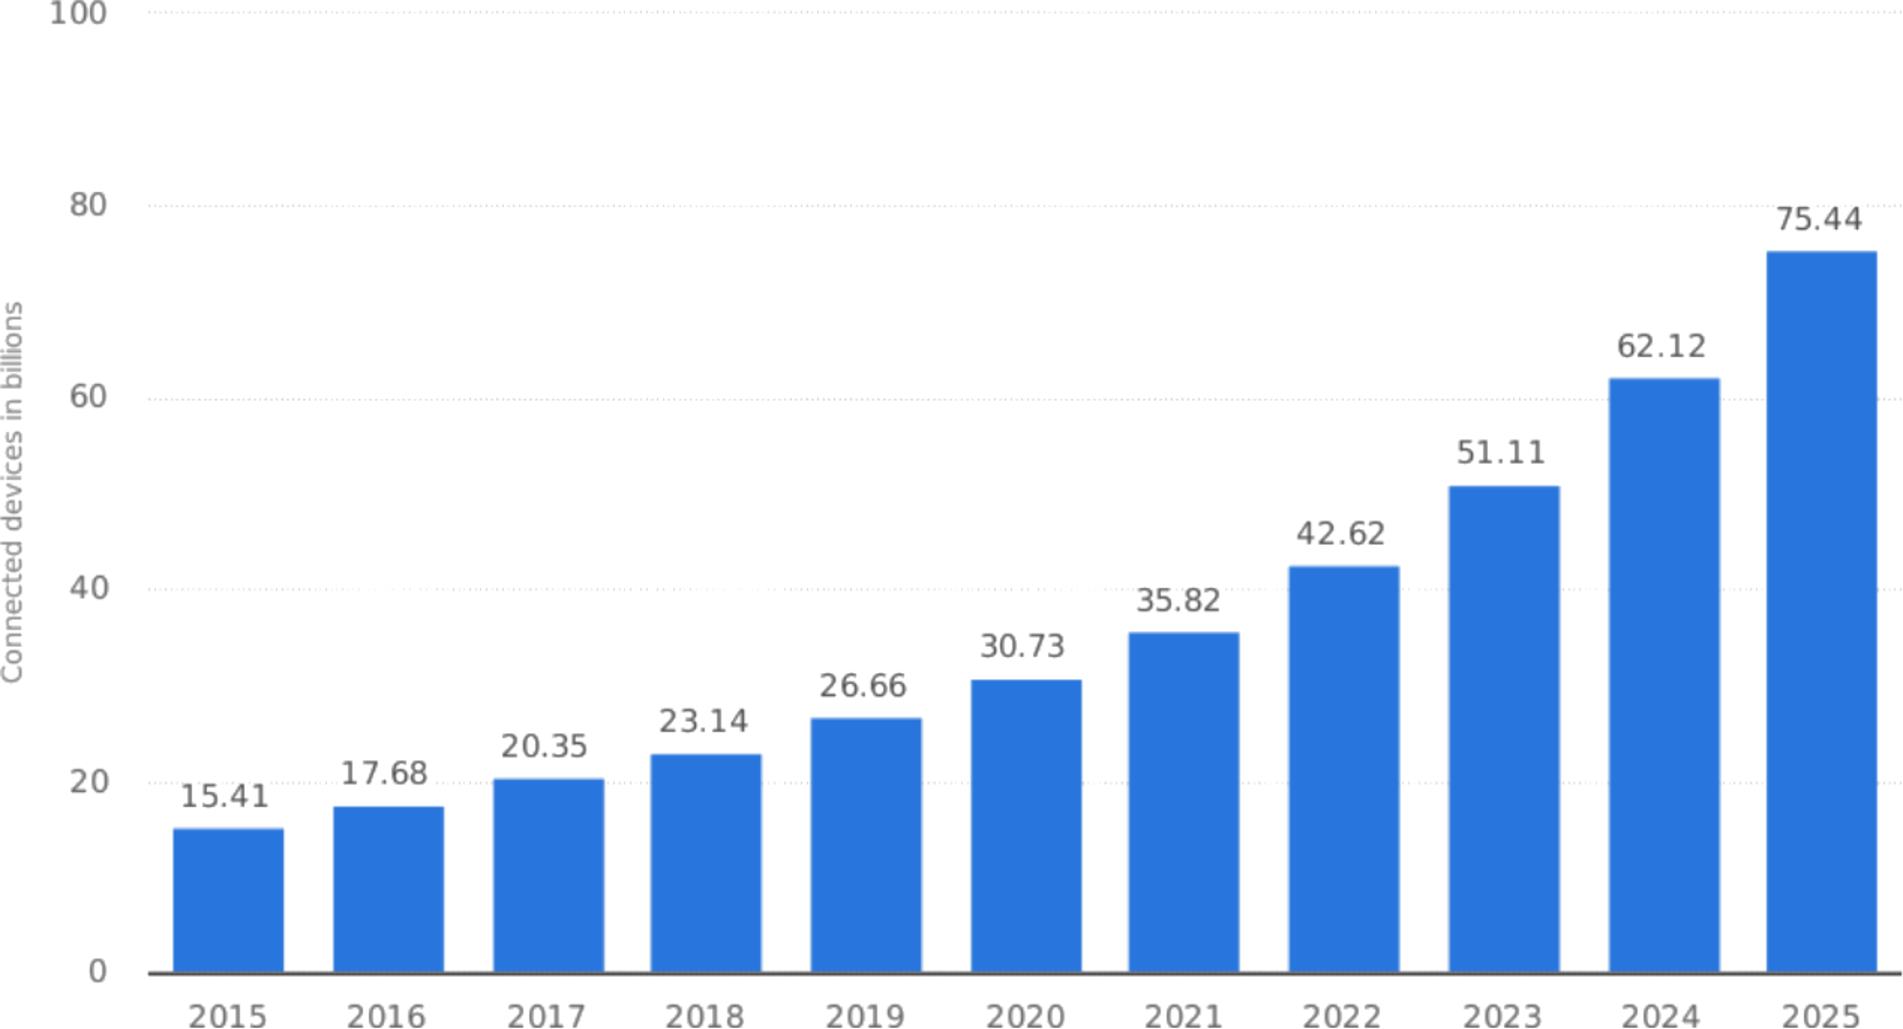
\includegraphics[width=0.8\linewidth]{img/iot_statistics.pdf}	
	\caption{Projected number of IOT devices worldwide}.
	\label{lit:fig:1}
\end{figure}

This change in communication strategy may seem inconsequential at first. However, upon deeper reflection in becomes clear that this is a major paradigm shift which brings IOT closer to the sensor network world it is often compared to. While the pioneering work in the IOT always assumed a one or two way communication between the IOT device and the cloud service, utilizing TCP/IP as an end-to-end protocol, it is becoming clear that this approach is unsustainable, and is often undesirable. This communication model has clear disadvantages in wasted communication, computation, and privacy. Furthermore the rigid computation communication model is not flexible enough to 
